% File: AI6103_Project.tex
%release 2023.0
\documentclass[letterpaper]{article} % DO NOT CHANGE THIS
\usepackage{aaai23}  % DO NOT CHANGE THIS
\usepackage{times}  % DO NOT CHANGE THIS
\usepackage{helvet}  % DO NOT CHANGE THIS
\usepackage{courier}  % DO NOT CHANGE THIS
\usepackage[hyphens]{url}  % DO NOT CHANGE THIS
\usepackage{graphicx} % DO NOT CHANGE THIS
\urlstyle{rm} % DO NOT CHANGE THIS
\def\UrlFont{\rm}  % DO NOT CHANGE THIS
\usepackage{natbib}  % DO NOT CHANGE THIS AND DO NOT ADD ANY OPTIONS TO IT
\usepackage{caption} % DO NOT CHANGE THIS AND DO NOT ADD ANY OPTIONS TO IT
\frenchspacing  % DO NOT CHANGE THIS
\setlength{\pdfpagewidth}{8.5in}  % DO NOT CHANGE THIS
\setlength{\pdfpageheight}{11in}  % DO NOT CHANGE THIS
%
% These are recommended to typeset algorithms but not required. See the subsubsection on algorithms. Remove them if you don't have algorithms in your paper.
\usepackage{algorithm}
\usepackage{algorithmic}
\usepackage{subcaption}
\usepackage{amsmath}
\usepackage{xcolor}
\usepackage{lettrine}

%
% These are are recommended to typeset listings but not required. See the subsubsection on listing. Remove this block if you don't have listings in your paper.
\usepackage{newfloat}
\usepackage{listings}
\DeclareCaptionStyle{ruled}{labelfont=normalfont,labelsep=colon,strut=off} % DO NOT CHANGE THIS
\lstset{%
	basicstyle={\footnotesize\ttfamily},% footnotesize acceptable for monospace
	numbers=left,numberstyle=\footnotesize,xleftmargin=2em,% show line numbers, remove this entire line if you don't want the numbers.
	aboveskip=0pt,belowskip=0pt,%
	showstringspaces=false,tabsize=2,breaklines=true}
\floatstyle{ruled}
\newfloat{listing}{tb}{lst}{}
\floatname{listing}{Listing}
%
% Keep the \pdfinfo as shown here. There's no need
% for you to add the /Title and /Author tags.
\pdfinfo{
/TemplateVersion (2023.1)
}

\setcounter{secnumdepth}{0} %May be changed to 1 or 2 if section numbers are desired.

% \iffalse
%Example, Multiple Authors, ->> remove \iffalse,\fi and place them surrounding AAAI title to use it
\title{Reproduction Of The Denoising Diffusion Probabilistic Model \\ AI6103 Project Report}
\author {
    % Authors
    Chen Zhitong (G2204728D),\textsuperscript{\rm 1}
    Fu Ziming (G2205212F),\textsuperscript{\rm 2}\\
    Luo Yiyang (G2204807B),\textsuperscript{\rm 3}
    Wang Xinyue (G2204921G),\textsuperscript{\rm 4}
}
\affiliations {
    % Affiliations
    s220166@e.ntu.edu.sg,\textsuperscript{\rm 1}
    zfu009@e.ntu.edu.sg,\textsuperscript{\rm 2}
    luoy0043@e.ntu.edu.sg,\textsuperscript{\rm 3}
    wang1913@e.ntu.edu.sg,\textsuperscript{\rm 4}
}
% \fi


% REMOVE THIS: bibentry
% This is only needed to show inline citations in the guidelines document. You should not need it and can safely delete it.
\usepackage{bibentry}
% END REMOVE bibentry

\begin{document}

\maketitle

% INTRODUCTION
\begin{abstract}
In this Project, we reproduce the model from the paper \textit{Denoising Diffusion Probabilistic Models}, which presents an innovative image denoising approach employing diffusion processes. The method iteratively denoises images, leveraging a probabilistic model to estimate noise distribution and enable effective noise reduction. We implement the DDPM and train the model for the task of human face image synthesis. The project code is available at \textcolor{blue}{https://github.com/MRTater/AI6103-Project}.
\end{abstract}

\section{Introduction}
\lettrine[lines=2, findent=3pt, nindent=0pt]{\textbf{T}}{he} \textit{Denoising Diffusion Probabilistic Models} (DDPM) represents a significant advancement in generative modeling, introducing an approach based on diffusion processes for iterative denoising. This method has demonstrated state-of-the-art (SOTA) performance in various image processing tasks, including image synthesis, super-resolution, and inpainting, making it a versatile tool for diverse applications. Additionally, DDPM has inspired the development of other diffusion-based models, such as Stable Diffusion, further expanding its impact on the field.

In this Project, we focus on reproducing the DDPM based on our understanding of the original paper. We adapt the network architecture to suit our limited computational resources without compromising performance. Furthermore, we incorporate strategies such as learning rate scheduling, skip connections, better activations, etc. to enhance model performance. Our implementation targets the task of human face image synthesis, utilizing the \textit{Synthetic Faces Dataset}\cite{david_beniaguev_2022} to train the model.

\section{Background}
Over the past few years, deep generative models have gained popularity due to their ability to learn complex data distributions, generate high-quality samples, and perform a wide range of tasks, such as image synthesis, inpainting, and translation. Examples of deep generative models include Variational Autoencoders (VAEs), Generative Adversarial Networks (GANs), and autoregressive models like PixelCNN.

Despite their success, these models face challenges. GANs struggle with generating high-quality samples and avoiding mode collapse, while autoregressive models are computationally expensive and time-consuming. Consequently, researchers have sought alternative approaches to address these limitations.

In this context, denoising score matching has garnered attention, leading to the development of DDPM. This alternative generative model addresses some of the shortcomings of VAEs and GANs by using a diffusion process to learn a noise model within a continuous-time framework.

DDPMs have emerged as a promising alternative to traditional generative models due to their high-quality training samples and stability. The DDPM approach simulates a reverse diffusion process, transforming a simple noise distribution into a complex data distribution through a series of denoising steps. A neural network describes the denoising process, learning to predict the noise added at each step of the diffusion process.

Additionally, the diffusion process used in DDPM has applications in other domains, such as optimization and machine learning, leading to new algorithms and techniques. This highlights the significant impact DDPM has had on the machine learning field and its potential to drive further advancements in the future.

% DATASET
\section{Dataset}
We chose the Synthetic Faces High Quality (SFHQ) Part 1 dataset, as shown in Figure \ref{fig:figure5}, for training our model. This dataset comprises 89,785 high-quality $1024 \times 1024$ curated face images created by "bringing to life" various artworks (paintings, drawings, 3D models) using a process similar to that described in a short Twitter thread. This process involves encoding the images into StyleGAN2 latent space and performing a minor manipulation that converts each image into a photo-realistic representation.

\begin{figure}[htbp]
\centering
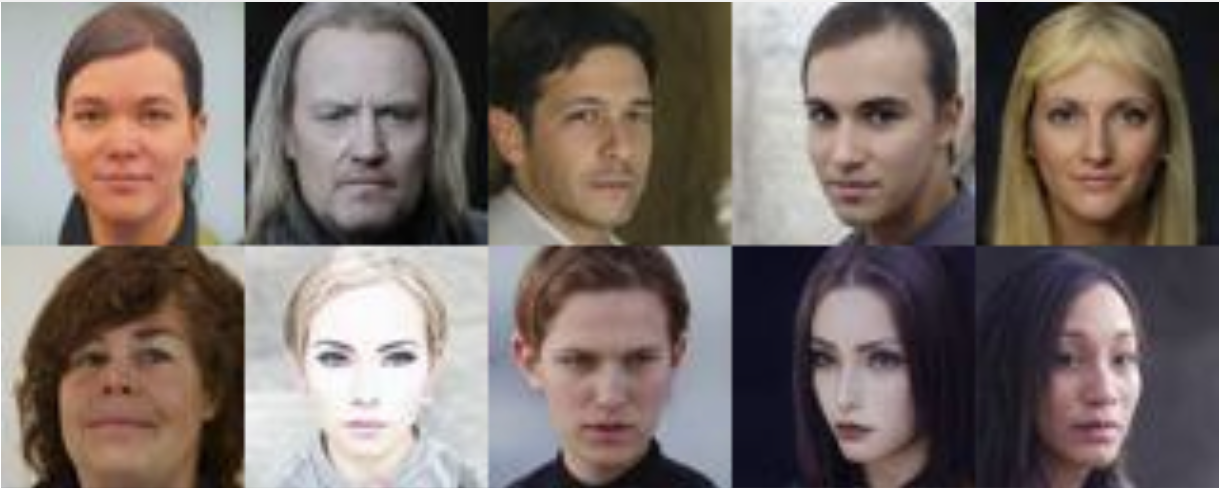
\includegraphics[width=0.88\linewidth]{f5.png} % Adjust the width and image file name as needed
\caption{Preview of the Synthetic Faces dataset.}
\label{fig:figure5}
\end{figure}

\subsection{Data Preprocessing}
Data preprocessing involves transforming raw data into a suitable range or scale that facilitates model learning. In our experiment, we performed several preprocessing steps on the data. Initially, we randomly selected 20,000 images from the dataset and resized them to 256 $\times$ 256 for our training set. To further accelerate training, given limited computational resources, we resized the images to 64 $\times$ 64 and applied a random horizontal crop as data augmentaion. The image data, which initially consisted of integers ranging from 0 to 255, was linearly scaled to the range of [-1, 1] to ensure compatibility with the model.

% ALGORITHM
\section{Diffusion Foward Process}
In the context of denoising diffusion probabilistic models (DDPM), the forward diffusion process, as described by Equation (1), is responsible for incrementally adding noise to the original image $x_0$ following a precise strategy at each timestep. This procedure aims to mimic the diffusion of the image across $T$ timesteps, generating a sequence of increasingly noisy images that ultimately converge to Gaussian noise.
\begin{equation}
q\left(x_{1: T} \mid x_0\right)=\prod_{t=1}^T q\left(x_t \mid x_{t-1}\right)
\end{equation}

The method of sampling noises is described by Equation (2). It is the conditional Gaussian noise with a mean that depends on the previous image and fixed variance, i.e., ($\beta_t I$) in our implementation. The sequence of betas is called the noise schedule, which describes how much noise is added at each timestep.
\begin{equation}
q\left(x_t \mid x_{t-1}\right)=N\left(x_t ; \sqrt{1-\beta_t} x_{t-1}, \beta_t I\right)
\end{equation}

Since the sum of Gaussian distributions is still a Gaussian distribution, as proven by Equation (3), given the set of betas, we can precompute various terms that will be employed in the forward diffusion process, such as the cumulative product of alphas ($\alpha^{cumprod}_t$), and 1 minus the cumulative product of alphas ($1-\alpha^{cumprod}_t$). These terms are utilized to control the variance and the noise introduced to the image at each timestep.
\begin{equation}
\begin{aligned}
& \mathrm{q}\left(\mathrm{x}t \mid x{t-1}\right)=\mathcal{N}\left(x_t, \sqrt{1-\beta_t} x_{t-1}, \beta_t I\right) \\
& =\sqrt{1-\beta_t} x_{t-1}+\sqrt{\beta_t} \epsilon \\
& =\sqrt{\alpha_t} x_{t-1}+\sqrt{1-\alpha_t} \epsilon \\
& =\sqrt{\alpha_t \alpha_{t-1}} x_{t-2}+\sqrt{1-\alpha_t \alpha_{t-1}} \epsilon \\
& =\sqrt{\alpha_t \alpha_{t-1} \alpha_{t-2}} x_{t-3}+\sqrt{1-\alpha_t \alpha_{t-1} \alpha_{t-2}} \epsilon \\
& =\sqrt{\alpha_t \alpha_{t-1} \cdots \alpha_1 \alpha_0} x_0+\sqrt{1-\alpha_t \alpha_{t-1} \ldots \alpha_1 \alpha_0} \epsilon \\
& q\left(x_t \mid x_0\right)=\mathcal{N}\left(x_t ; \sqrt{\alpha_t} x_0,\left(1-\bar{\alpha}_t\right) I\right) =\sqrt{\bar{\alpha}_t} x_0+\sqrt{1-\bar{\alpha}_t} \epsilon
\end{aligned}
\end{equation}

\subsection{Beta Scheduling}
The choice of the beta schedule has a significant impact on the performance of the DDPM. We propose two beta schedules: linear and cosine. \\\\
The linear beta schedule is defined as Equation (4):

\begin{equation}
\beta_t = \text{start} + \frac{t (\text{end} - \text{start})}{T},
\end{equation}

\noindent where $T$ is the total number of timesteps, and start and end are the initial and final values of the beta schedule.

\noindent The cosine beta schedule is defined as Equation(5):
\begin{equation}
\begin{aligned}
\bar{\alpha}_t &= \frac{f(t)}{f(0)}, \quad f(t) = \cos \left(\frac{t / T+s}{1+s} \cdot \frac{\pi}{2}\right)^2, \\
\beta_t &= 1-\frac{\bar{\alpha}_t}{\bar{\alpha}_{t-1}} \qquad
\end{aligned}
\end{equation}

The cosine beta schedule features a linear drop-off of $\bar{\alpha}_t$ in the middle while maintaining stable noise levels near $t = 0$ and $t = T$as shown in Figure \ref{fig:figure1}. This provides a more gradual noise addition compared to the linear schedule. A small offset $s$ is introduced to avoid overly small $\beta_t$ values near $t = 0$. The schedule is defined using the cosine function, ensuring smooth noise transitions. By clipping beta values to a maximum limit, it prevents excessive noise and improves denoising performance, especially for lower resolution images.

\begin{figure}[htbp]
    \centering
    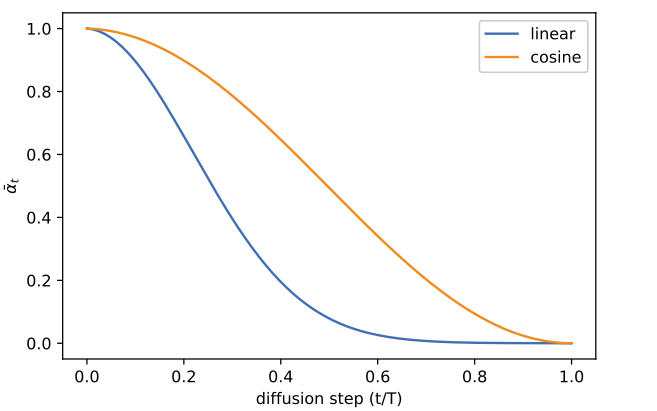
\includegraphics[width=0.88\linewidth]{f1.png} % Adjust the width and image file name as needed
    \caption{Linear and cosine beta schedules}
    \label{fig:figure1}
\end{figure}

\subsection{Summary of the Forward Process}
The forward diffusion process for a specific timestep $t$ can be described as follows:
\begin{enumerate}
\item Sample Gaussian noise $\epsilon \sim \mathcal{N}(0, 1)$ with the same dimensions as the input image $x_0$.
\item Compute the noisy image $x_t$ as Equation(4):
\begin{equation}
    x_t = \sqrt{\alpha^{cumprod}_t} x_0 + \sqrt{1 - \alpha^{cumprod}_t} \epsilon,
\end{equation}
\noindent where $\alpha^{cumprod}_t$ and $1 - \alpha^{cumprod}_t$ govern the mean and variance of the noise introduced to the image, respectively. The noisy image is then clamped to the range $[-1, 1]$ to ensure valid pixel values.
\end{enumerate}

The forward diffusion process is applied iteratively for all $T$ timesteps as shown in Figure \ref{fig:figure2}, producing a sequence of increasingly noisy images. During training, the DDPM model learns to invert this process by predicting the noise added at each timestep, enabling it to synthesize new images by denoising Gaussian noise in the later part.

\begin{figure}[htbp]
    \centering
    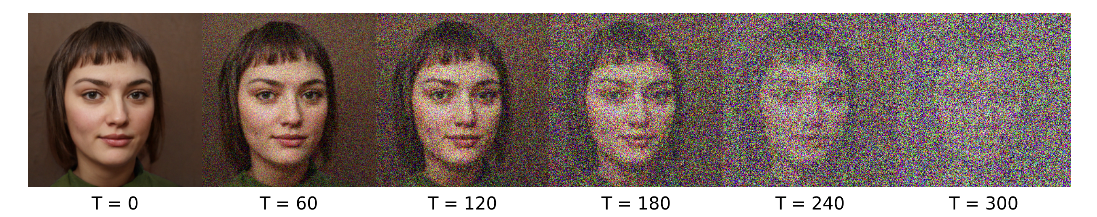
\includegraphics[width=0.88\linewidth]{f2.png} % Adjust the width and image file name as needed
    \caption{A preview of forward diffusion process by time steps T}
    \label{fig:figure2}
\end{figure}

\section{Parametrized Backward Process}
The backward process in denoising diffusion probabilistic models (DDPM) is responsible for reconstruct the image $x_0$ back from the noisy image at the final timestep $x_T$. This process, parametrized by $\theta$, is described by Equation (9):
\begin{equation}
\begin{aligned}
p_\theta\left(x_{0: T}\right)=p\left(x_T\right) \prod_{t=1}^T p_\theta\left(x_{t-1} \mid x_t\right)\\
x_{t-1} \approx x_t-\text { noise }
\end{aligned}
\end{equation}

The parametrized backward process is learned by the DDPM using a neural network, in our case, a simplified variant of the U-Net, along with sinusoidal position embeddings for the information of time steps. Notice that we only learn the mean, since the variance is fixes as mentioned.

\subsection{U-Net}
The U-Net serves as the core of the parametrized backward process in denoising diffusion probabilistic models. Its ability to capture both local and global information makes it ideal for denoising tasks.

The architecture maintains a large receptive field and preserves spatial information throughout the processing, enabling detailed image generation.  

We use a simplified version of U-Net as shown in Figure \ref{fig:figure3}, named SimpleUnet, consisting of an initial convolutional layer, a series of downsampling and upsampling blocks, and an output convolutional layer. The blocks incorporate time embedding and consist of convolutional layers, batch normalization layers, and activation functions.

The SimpleUnet is initialized with customizable settings like activation function (ReLU or SiLU), self-attention, and skip connections.
Skip connections link corresponding downsampling and upsampling layers, propagating detailed spatial information to reconstruct denoised images more accurately. Additionally, there are skip connections within the blocks themselves, allowing for better information flow. The architecture has 5 downsampling and upsampling layers, with channels reaching up to 1024 in the middle layers. This structure captures hierarchical input image representations, including both high-level and low-level features.

\begin{figure*}[htbp]
    \centering
    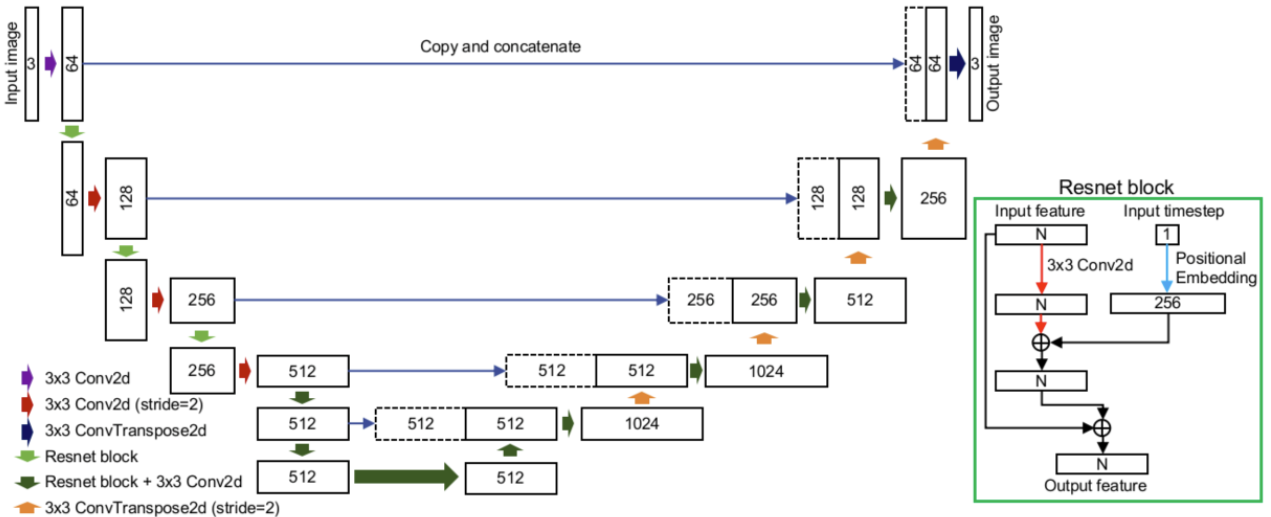
\includegraphics[width=0.8\linewidth]{f3.png} % Adjust the width and image file name as needed
    \caption{The SimpleUnet}
    \label{fig:figure3}
\end{figure*}

\subsection{Sinusoidal Position Embeddings}
Incorporating temporal information is crucial in denoising diffusion probabilistic models (DDPM). To achieve this, we employ sinusoidal position embeddings, which provide a continuous and differentiable representation of time.

Sinusoidal position embeddings are computed using the following formulae:
\begin{equation}
\begin{aligned}
P(k, 2 i)=\sin \left(\frac{k}{n^{2 i / d}}\right) \\
P(k, 2 i+1)=\cos \left(\frac{k}{n^{2 i / d}}\right)
\end{aligned}
\end{equation}

Where $P$ represents the position embedding matrix, $k$ is the time step, $n$ is a constant (typically 10000), $d$ is the dimensionality of the embeddings, and $i$ is an index that ranges from 0 to $\frac{d}{2} - 1$. These equations generate sine and cosine functions with different frequencies, effectively encoding temporal information within the embeddings.

The resulting sinusoidal embeddings as shown in Figure \ref{fig:figure8}, can be used within the DDPM, effectively encoding temporal information for the denoising process. The sinusoidal nature of these embeddings ensures that they can be easily combined with other representations, facilitating the learning process for the model.

\begin{figure}[htbp]
    \centering
    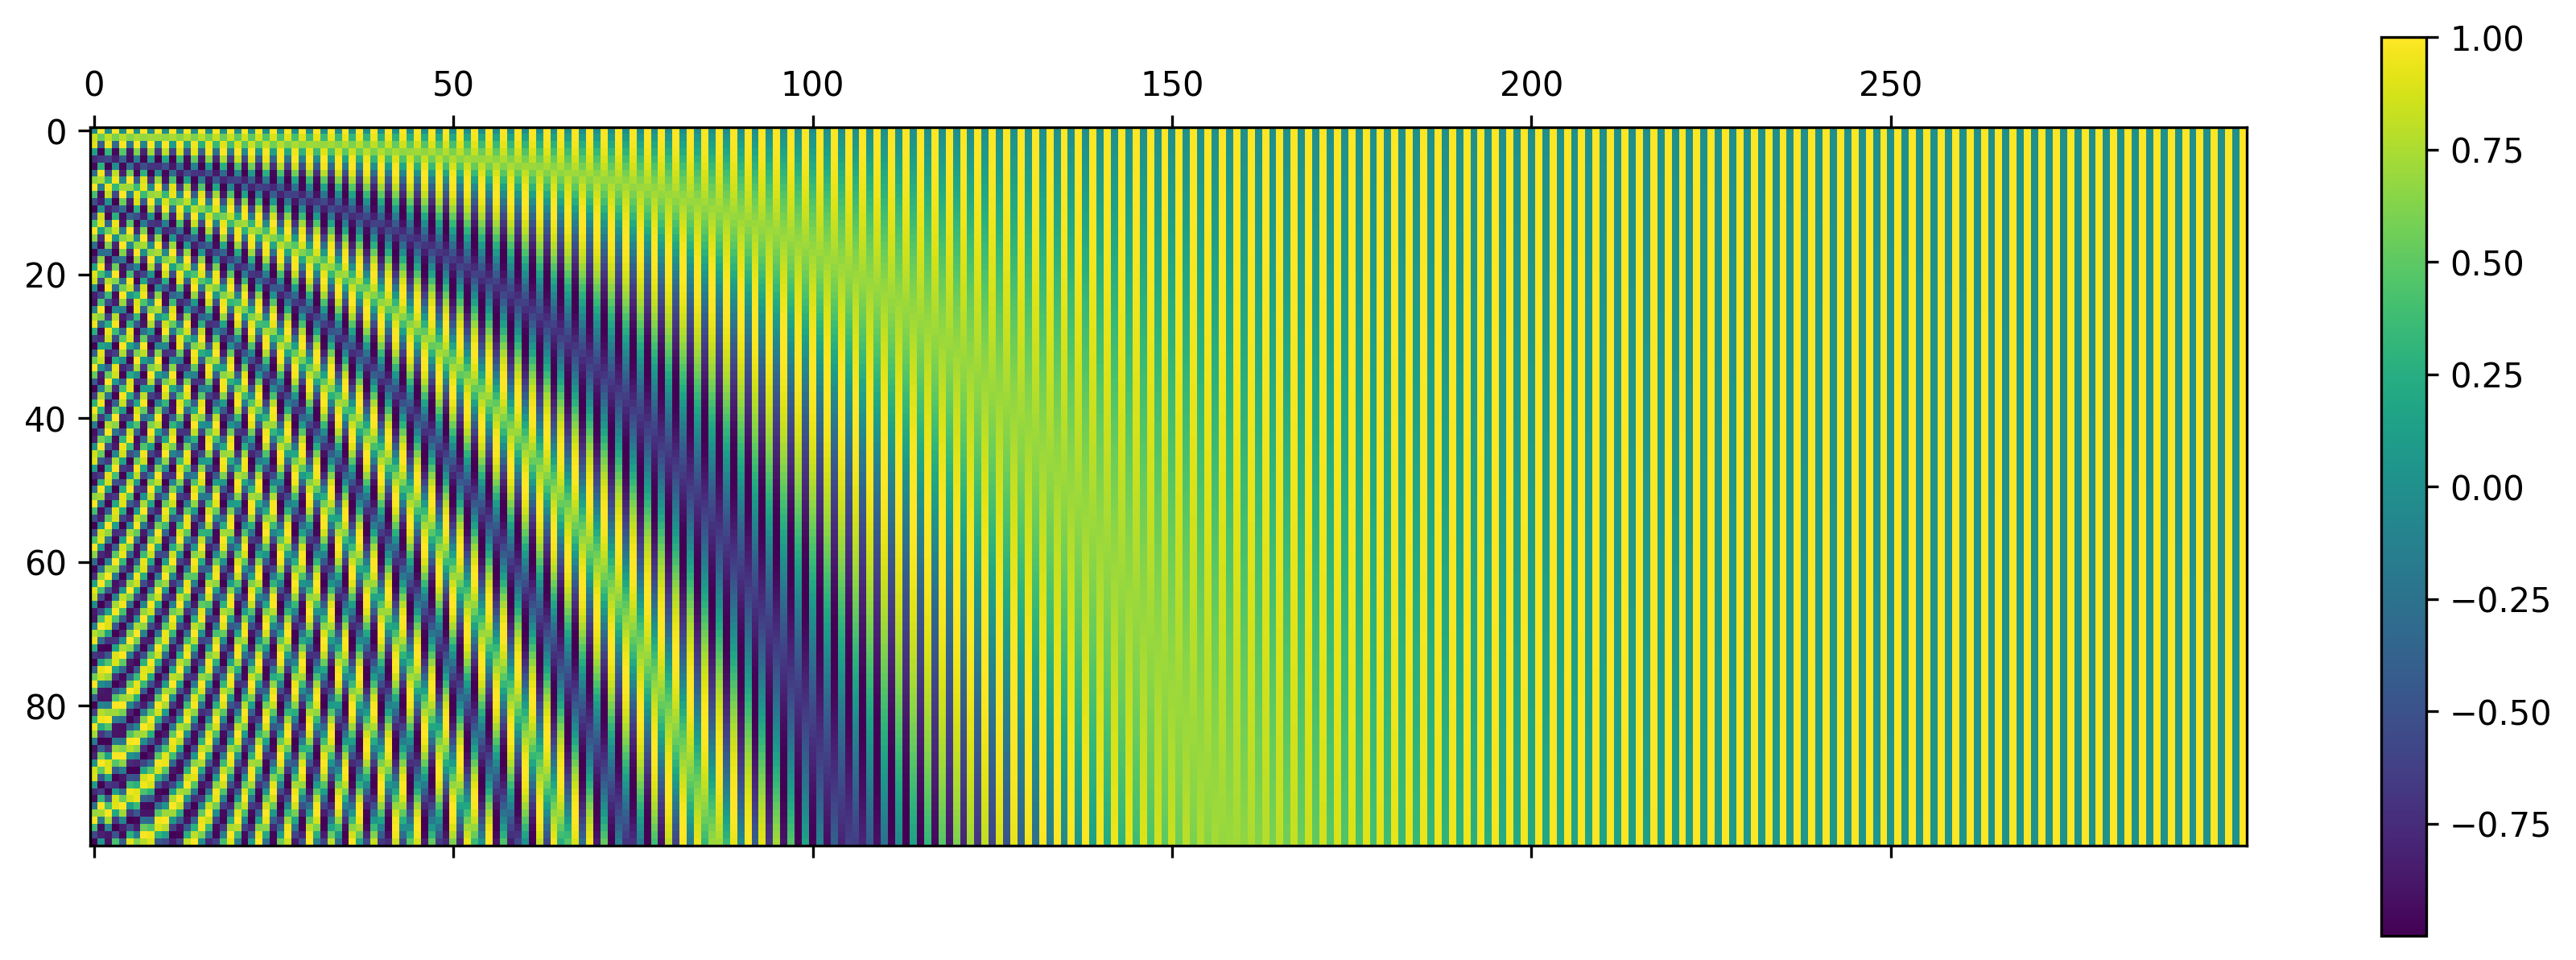
\includegraphics[width=1.0\linewidth]{f8.png} % Adjust the width and image file name as needed
    \caption{Position embeddings, T=300}
    \label{fig:figure8}
\end{figure}

\subsection{Loss Function}
In the DDPM, the loss function is used to measure the discrepancy between the actual noise and the predicted noise at each timestep during training. Here, we present two different loss functions: L1 and L2.\\

\noindent The L1 loss function is defined as follows:
\begin{equation}
\mathcal{L}{\text{1}}(\theta) = \sum_{t=0}^{T-1} \lVert \epsilon_t - \text{model}(x_t, t) \rVert_1,
\end{equation}
    
\noindent The L2 loss function, also known as the Mean Squared Error (MSE) loss, can lead to smoother denoising results as it tends to penalize large deviations more heavily. It is defined similarly to the L1 loss:
\begin{equation}
\mathcal{L}{\text{2}}(\theta) = \sum_{t=0}^{T-1} \lVert \epsilon_t - \text{model}(x_t, t) \rVert_2^2,
\end{equation}

\noindent where $\epsilon_t$ is the true noise, $x_t$ is the noisy image, $t$ is the timestep, and $\text{model}(x_t, t)$ is the predicted noise at timestep $t$.

During training, either the L1 or L2 loss can be used to optimize the model, depending on the desired denoising characteristics.

\subsection{Summary of the Backward Process}
The parametrized backward process in DDPM sythesize the original image $x_0$ from the noisy image $x_T$. The process involves a simplified U-Net architecture and sinusoidal position embeddings for encoding temporal information.
\begin{enumerate}
\item Perform batch training with noisy images $x_T$ and corresponding time steps.
\item Encode time steps using sinusoidal position embeddings to generate a position embedding matrix $P$.
\item Process input images using the SimpleUnet and feed in with the sinusoidal position embeddings to incorporate temporal information in the denoising process.
\item Iterate through the training process, adjusting model parameters to minimize the loss function and refining the denoising capability.
\item By following these steps, the parametrized backward process effectively synthesizes the original images from the noisy counterparts, improving the performance of the denoising diffusion probabilistic model.
\end{enumerate}

\section{Metric}
Considering that our project focuses on the task of image synthesis, we choose the \textit{Fréchet Inception Distance} (FID) as the metric for our task. FID is a widely-used metric for evaluating the quality of generated images. First introduced by Martin Heusel et al. in 2017, FID measures the similarity between distributions of generated and real images in the feature space of a pre-trained Inception-v3 neural network.

The principle behind FID for calculating image distance can be summarized as follows: given that a random variable follows a Gaussian distribution, the distribution can be determined by its mean and variance. Two distributions are considered identical if their means and variances are the same. In the case of multidimensional distributions, the covariance matrix is used to measure the correlation between dimensions. Thus, FID employs the mean and covariance matrix to calculate the distance between two distributions.

The FID score can be calculated using the following steps:
\begin{enumerate}
\item Extract feature vectors from the real and generated images using a pre-trained Inception-v3 neural network.
\item Calculate the mean and covariance of the feature vectors separately for the real and generated images.
\item Compute the Fréchet distance between the two distributions.
\end{enumerate}

The mathematical formula for FID is expressed as Equation 11. Here, $\mu_x$ and $\mu_y$ represent the feature-wise means of the real and generated images, and $\Sigma_x$ and $\Sigma_y$ denote the covariance matrices of the real and generated feature vectors.
\begin{equation}
\operatorname{FID}(x, g)=\left|\mu_x-\mu_g\right|_2^2+\operatorname{Tr}\left(\Sigma_x+\Sigma_g-2\left(\Sigma_x \Sigma_g\right)^{\frac{1}{2}}\right)
\end{equation}

By improving the FID score, our model aims to generate images that are more similar to the real images in terms of their feature distributions, resulting in higher quality synthesized images.

\section{Experiments}
For all experiments, we set $T = 300$. We chose forward process variances as constants, increasing linearly from $\beta_1=10^{-4}$ to $\beta_T=0.02$, consistent with the original paper's settings. The size of the sampled images is $64 \times 64$.

We employed a U-Net backbone as the primary network, illustrated in Figure \ref{fig:figure3}. Parameters are shared across time, specified to the network using sinusoidal position embeddings from the Transformer architecture.

In addition, we implemented a cosine $\beta$ schedule for further investigation of the diffusion model.

Due to computational constraints, we omitted the self-attention layer as it was deemed too computationally expensive.

\subsection{Sampling Process}
The sampling process in our experiments involves reversing the diffusion process. By starting with pure noise as input, the model iteratively removes noise until a realistic image is generated. In the context of the diffusion model, the sampling process is essentially equivalent to denoising.

We sampled 64 $\times$ 64 images using our diffusion model in our experiments. Our implementation achieved a generation speed of 25.7 seconds per batch, with each batch containing 128 images. Table \ref{tab:FID} presents the FID scores on the Synthetic Faces High Quality (SFHQ) part 1 dataset, where the FID score decreases with the number of training epochs. Figure \ref{fig:figure7} illustrates the loss decreasing with the number of training epochs, indicating that our model's ability to generate high-quality images improves as training progresses. Some generated results are showcased in Figure \ref{fig:high}.

\begin{table}[t]
\centering
\begin{tabular}{c|c}
\textbf{Epochs} & \textbf{FID} \\
\hline
        200  & 233.36 \\
        300  & 220.25 \\
        450 & 198.03
\end{tabular}
\caption{SFHQ Results, measured with FID}
\label{tab:FID}
\end{table}

\begin{figure}[htbp]
    \centering
    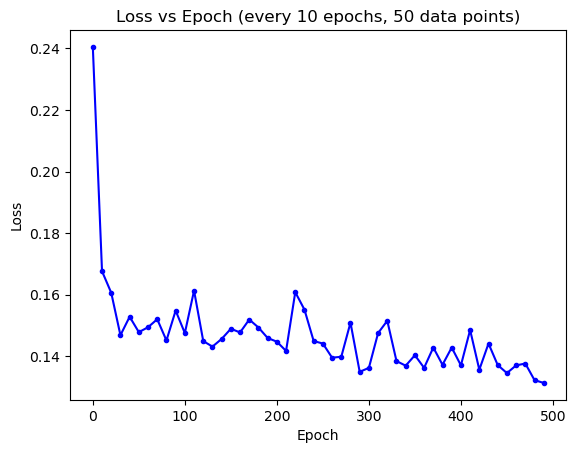
\includegraphics[width=0.45\textwidth]{f6.png} % Adjust the width and image file name as needed
    \caption{Loss vs Epoch, T=300}
    \label{fig:figure7}
\end{figure}

\begin{figure}[htbp]
    \centering
    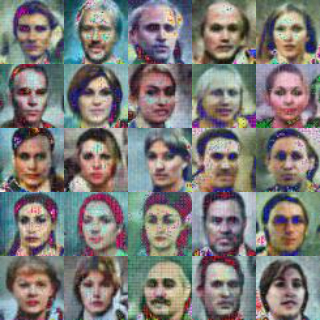
\includegraphics[width=0.45\textwidth]{f7.jpg}
    \caption{SFHQ samples, FID=198.03}
    \label{fig:high}
\end{figure}

\subsection{Beta Scheduler}
For our experiments, we employed both linear and cosine $\beta$ schedules to investigate their impact on the model's performance.

Our results revealed that the cosine schedule outperformed the linear schedule in terms of sample quality and training stability, as illustrated in Figure \ref{fig:figure4}. Specifically, the cosine schedule yielded lower FID scores compared to the linear schedule.

In conclusion, we determined that the cosine $\beta$ schedule is a more effective approach for training our diffusion model than the linear schedule. Its smoother and more gradual transition between values facilitates enhanced performance and stability during the training process.

\subsection{Activation Function}
We conducted experiments to investigate the impact of two different activation functions on the performance of our model: SiLU and ReLU as shown in Table \ref{tab:act}.

Our results indicate that the choice of activation function does not significantly influence the model's performance. Specifically, we observed that employing SiLU as the activation function resulted in a slight improvement in the model's accuracy, while ReLU demonstrated a marginally better convergence speed.

\begin{table}[t]
    \centering
    \begin{tabular}{c|c}
    \textbf{Activations} & \textbf{FID} \\
    \hline
            SILU  & 233.36 \\
            RELU  & 235.13
    \end{tabular}
    \caption{Comparison between activations, measured by FID, epoch=200}
    \label{tab:act}
    \end{table}

\begin{figure}[htbp]
    \centering
    \begin{subfigure}{0.45\textwidth}
        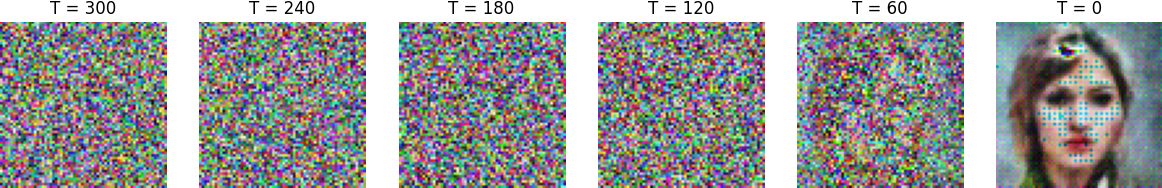
\includegraphics[width=\textwidth]{f4.jpg}
        \caption{64*64, T=300, linear, FID=237}
        \label{fig:figure4a}
    \end{subfigure}
    \hfill
    \begin{subfigure}{0.45\textwidth}
        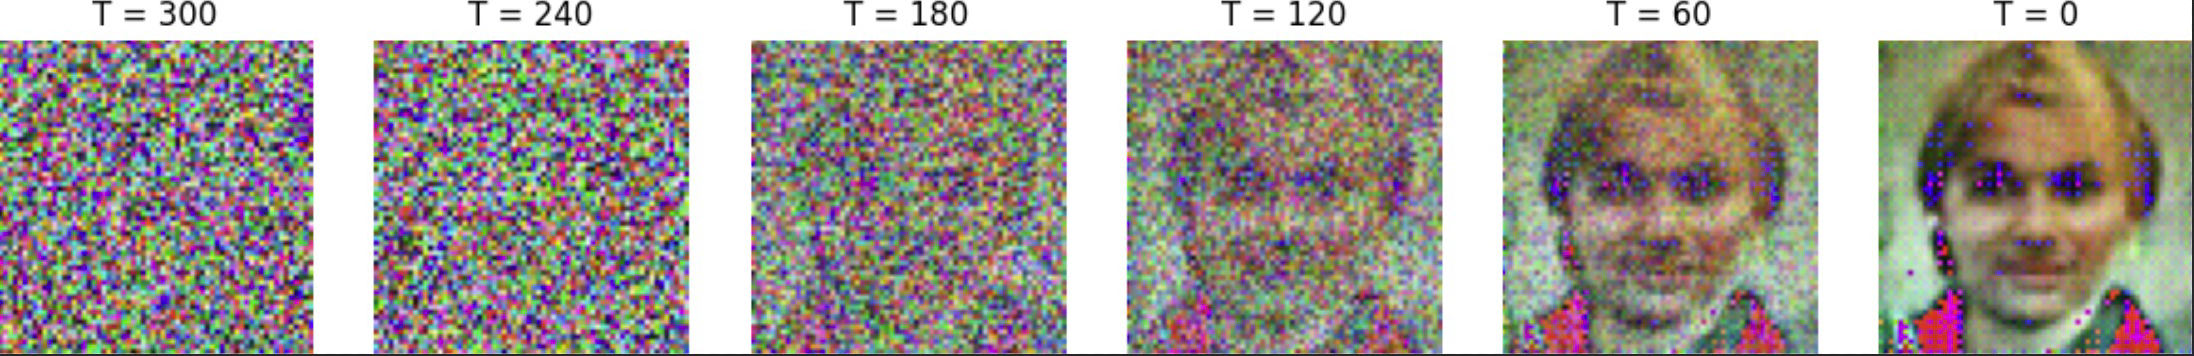
\includegraphics[width=\textwidth]{f9.png} % Replace with the correct file name
        \caption{64*64, T=300, cosine, FID=220.25} % Replace with the correct caption
        \label{fig:figure4b}
    \end{subfigure}
    \caption{Comparison of synthesized images via backward process with different beta scheduler: (a) linear; (b) consine.}
    \label{fig:figure4}
\end{figure}

\subsection{Result Analysis}
Our model was only able to generate images with an FID score of around 200, which is less realistic than the results reported in the original paper. Moreover, some noise and color jittering can be observed in the generated images, indicating that the model's denoising ability could be further improved. There are several factors that might have negatively impacted our model's performance.

One such factor is that, in contrast to the original paper, which employed CelebA-HQ models with 114 million parameters \cite{2020denoising}, we utilized a much shallower network consisting of only 62 million parameters. Shallower networks, with fewer layers and parameters, can constrain the model's learning ability. In the context of our diffusion model, this means that the model may exhibit inferior performance in learning noise distributions, thereby generating lower-quality images. Self-attention layers facilitate the model's focus on crucial information and relationships, which can enhance the accuracy of the diffusion process. Eliminating self-attention layers may impair the model's capacity to capture features of noise distribution and the relationships within different feature maps, ultimately diminishing the model's denoising ability.

Furthermore, we opted for a smaller value of $T = 300$, as opposed to the original paper's $T = 1000$ \cite{2020denoising}. Although this choice facilitated training, it adversely affected the generation process. Employing a smaller T value can impact the diffusion results in several ways:

\begin{itemize}
\item \textbf{Reduced Quality}. Using a smaller T value truncates the diffusion process, leading to lower-quality image or data generation. The resulting images or data may contain artifacts or appear blurry, which might be undesirable in certain applications.
\item \textbf{Limited Detail}. A smaller T value also restricts the amount of detail in the generated images or data. Consequently, the generated images or data may lack fine-grained detail compared to those produced with a larger T value.
\item \textbf{Limited Diversity}. The diversity of the generated images or data might also be compromised when using a smaller T value. Images or data generated with a smaller T value may be less diverse and exhibit a narrower range of features or characteristics.
\end{itemize}

Additionally, we selected a relatively modest epoch setting, which could have potentially affected the model's performance. Initially, we assumed that the epoch settings would not significantly influence the experiment's outcome beyond a certain timestep (200 in our experiment), considering that the loss remained relatively stable. However, upon examining the results, we observed that the FID of the generated images varied considerably compared to the change in loss, suggesting that longer epochs might be necessary to optimize the model's performance. This could be attributed to the limited learning capacity of our model.

In summary, our model's ability to generate realistic images was limited, with generated images only attaining an FID score of approximately 200 and exhibiting noise and color jittering. Factors that adversely affected the model's performance included using a shallower network with fewer parameters than the original paper, a smaller T value, and a relatively modest epoch setting.

\section{Conclusion}
In summary, our reimplementation of the DDPM has generated image samples comparable to those in the original paper, demonstrating its effectiveness as a powerful generative model. Although our implementation was adapted to accommodate limited computational resources, it has underscored the significant potential of the DDPM for generative tasks. Furthermore, recent advances such as Stable Diffusion have bolstered the performance of diffusion-based models in this domain, highlighting the potential of incorporating DDPM into various generative models and machine learning systems. As research into DDPM's capabilities progresses, we expect to uncover novel applications and deepen our understanding of this promising approach, paving the way for further advancements in the field.

\bibliography{aaai23}

\end{document}


